\chapter{Prosessdokumentasjon}
%\marginpar{
%Test for sitering av kilder.\cite{forelesning:tulpesh}\cite{book:utforming}\cite{book:desintsystems}
%}
\lettrine[lines=2]{F}{} ølgende kapittel beskriver hvordan hele utviklingsprosessen av prototypene har foregått og som illustrerer hele prosessen fra idé til mockup til hi-fi prototype. Kapittelet består av mange bilder og illustrasjoner for å på enklest mulig måte illustrere prosessen. For eventuell beskrivelse av funksjonalitet av de modulene som er synlige på bildene henvises det til appendiks \ref{app:funksjonalitet}.




\section{Første utkast} \label{sec:utkast}
%\marginpar{Viktige prinsipper:
%feedback, constraints (bruker får ikke gjøre feil), affordances
%}
%\marginpar{Husk at vi borde ta med en navigasjonkart}
%\marginpar{Støtteord:
%Usability (brukbarhet): konsistens, brukerkontroll, passende presentasjon.
%}
Etter at idéen om hva prosjektet skulle handle om tok det ikke lang tid før det ble enighet om som skulle inngå i løsningen. Det er i stor grad lagt vekt på at løsningen følger \textit{Gestalt}-prinsipper som en underliggende tommelfingerregel for en god design og layout.
Systemet skulle kunne administreres via nettleser som gjør det mulig å bruke systemet fra hvilken som helst maskin og med noen tilpasninger også fra nettbrett eller telefon.
På det tidspunktet handlet diskusjonen om hvordan man skulle fordele de forskjellige modulene og funksjonalitetene på så få hovedområder som mulig, der hvert av de områdene blir et element i hovedmenyen. 
I det første utkastet bestod disse av totalt fem forskjellige seksjoner som presenteres i tabell \ref{tab:sidekart}.
%\begin{center}
%\texttt{Editorer | Meldinger | Resurser | System | Servere}
%\end{center}
\begin{table}[h]
\caption[Sidekart]{Enkelt sidekart over det første utkastet. Tabellhode representerer hver enkel menykategori. I rad to presenteres forslag til hver menykategori.}
\label{tab:sidekart}
\newcommand{\paddA}{0.5ex}
\newcommand{\paddB}{0.2ex}
\renewcommand{\familydefault}{\ttdefault}\normalfont
\begin{tabularx}{\textwidth}{|*5{>{\centering\arraybackslash}X|}@{}|}
\hline
\vspace*{\paddA} Editorer & \vspace*{\paddA} Ressurser & \vspace*{\paddA} Meldinger & \vspace*{\paddA} System & \vspace*{\paddA} Servere \\[2ex] 
\hline
\vspace*{\paddB} Java		&	\vspace*{\paddB} HTML Val			& 	\vspace*{\paddB} Ny 	& 	\vspace*{\paddB} Apache 	& \vspace*{\paddB} Brannmur \\
HTML \& PHP		& 	CSS Val		 	& 		Les		& 	MySQL 	& Brukerg \\
MySQL	& 	W3Schools 		& 				& 	SSH 		& Logg \\
C/C++/C\# 		& 	DropBox 			& 				& 			& Filbehnadling \\
 		& 	Terminal 		& 				& 			& Systeminfo \vspace*{0.2ex} \\

\hline
\end{tabularx} 
\end{table}

Idéen ble deretter tegnet i form av en iterativ prosess. Det ble til slutt enighet om et resultat for idéen som ble godkjent for å bygge videre på. Skissen presenteres i figur \ref{fig:foersteutkast}.
\begin{figure}[h]
%bruk \begin{figure}[ht] dersom figuren ikke skal flyte
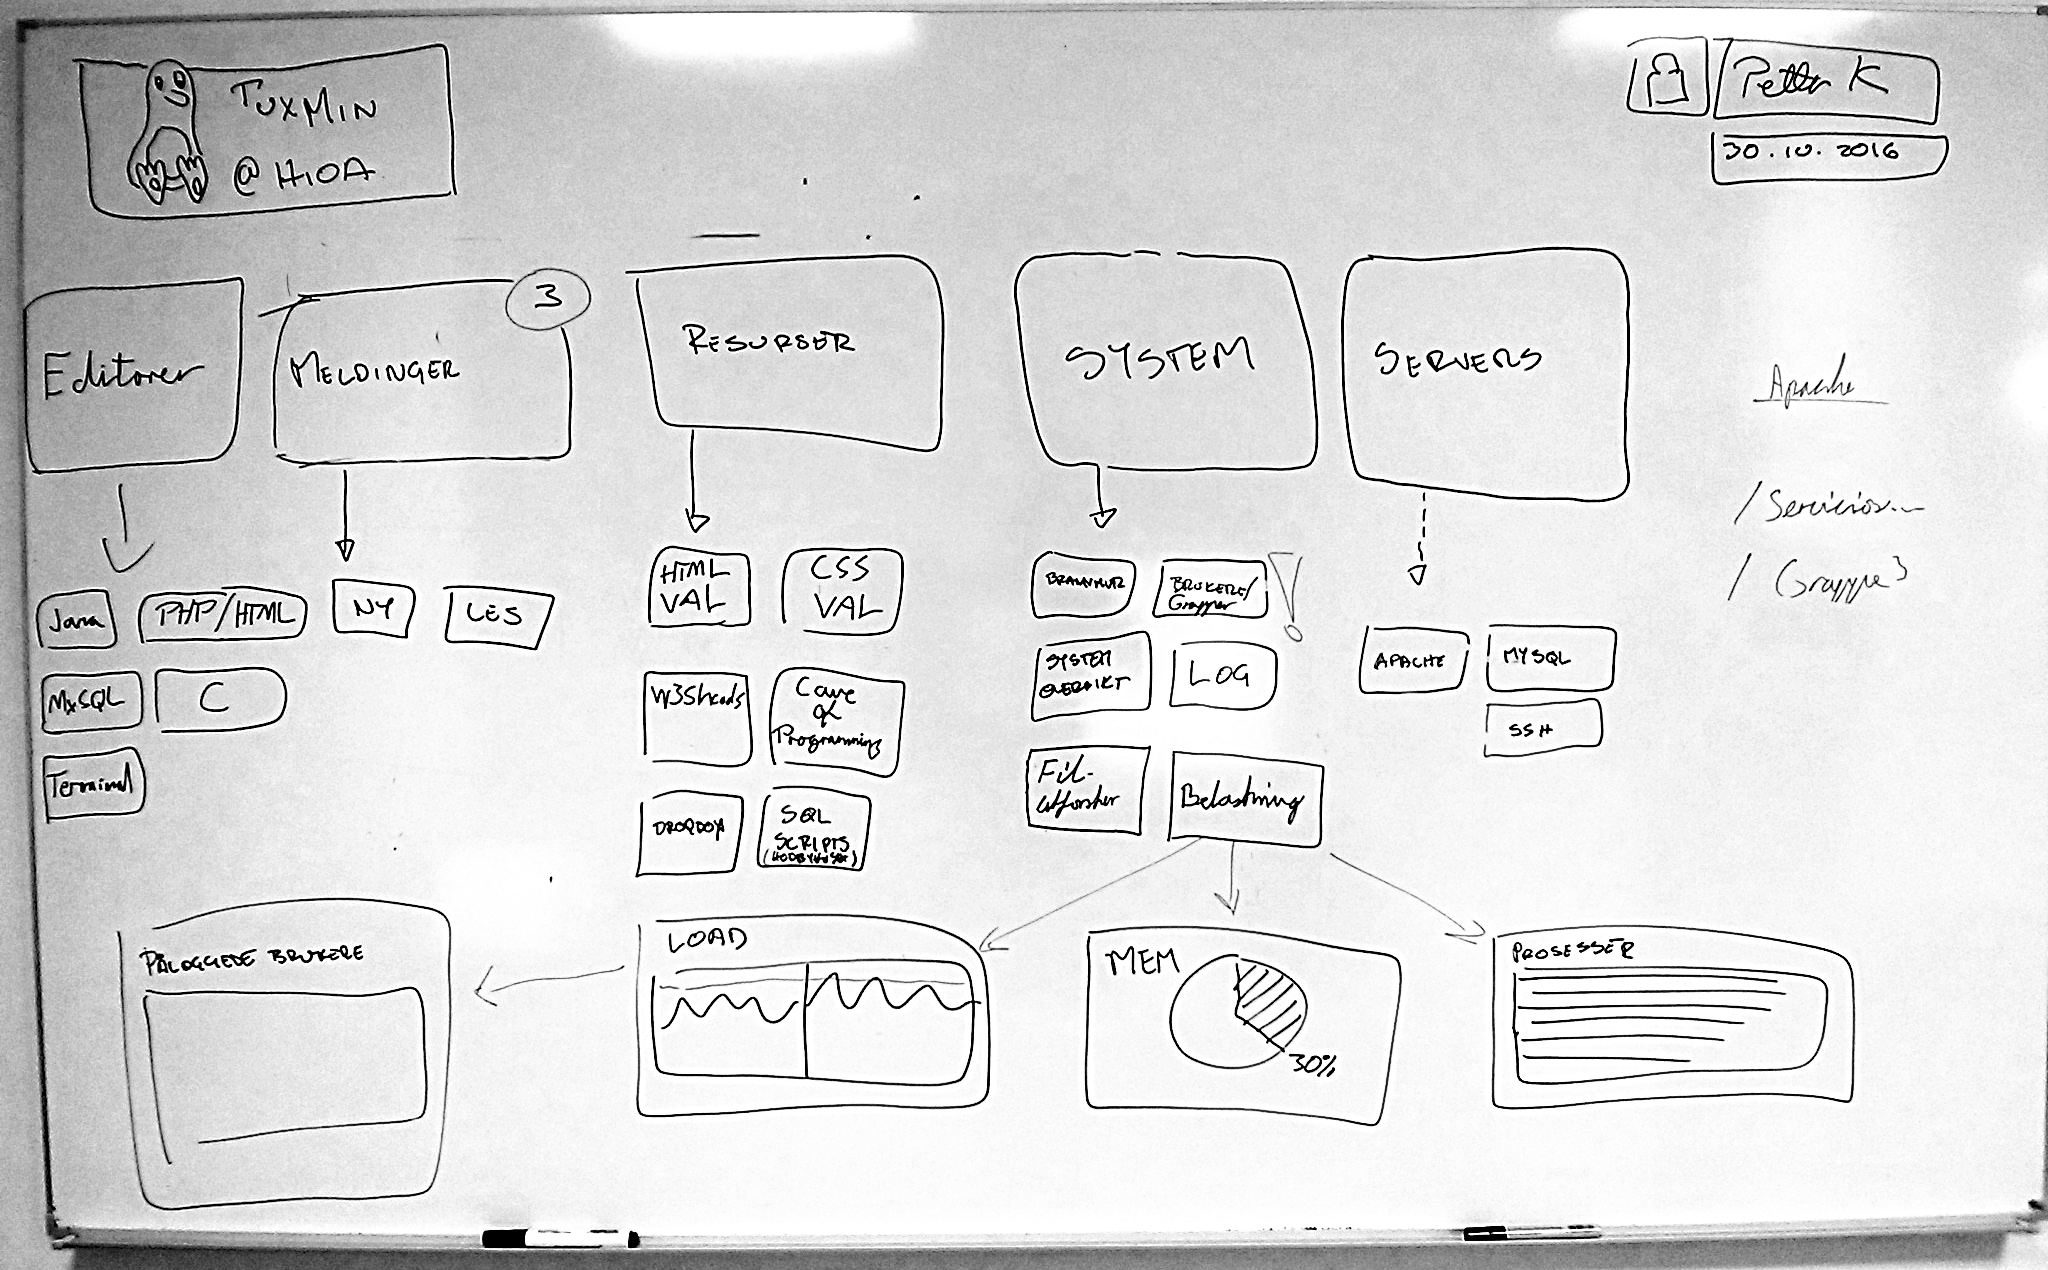
\includegraphics[width=\textwidth,height=\textheight,keepaspectratio]{./img/prosessdokumentasjon/foersteutkast/foerste.jpg}
\caption[Første utkast]{Første utkast over brukergrensesnittet.}
\label{fig:foersteutkast}
\end{figure}

\section{Low-fi prototype} \label{sec:lowfi}
\emph{Avsnittet inneholder et stort antall mockups som representerer forskjellige skjermbilder. Det er flere bilder som er plassert i teksten, og dersom noen av komponentene i bildene oppleves for små, er samtlige av bildene presentert i høyere oppløsning i appendiks \ref{sec:appendiksLowFi} side \pageref{sec:appendiksLowFi}.}

Det er ganske vanlig at man til en low-fi prototype bruker papp eller papir for å visualisere hvordan man kan bruke en GUI. I dette prosjektet ble det benyttet \href{http://balsamiq.com/products/mockups/}{\textit{Balsamiq Mockups}} som ga mulighet til å ikke bare visualisere hvordan brukergrensesnittet skulle se ut men også legge inn enkel funksjonalitet. Blant annet at man fikk mulighet til å klikke seg videre til neste skjermbilde direkte ved å trykke på fra menyer eller knapper i mockupen (en linkbasert mockup \cite{book:utforming}). Dette resulterte i en god følelse over hvordan det ville være å bruke det ferdige grensesnittet.

Dersom man tar et raskt overblikk over framsiden i figur \ref{fig:lowfi_fremside} ser man at menyen er gruppert etter gestalt prinsipper for proksimitet og likhet.\cite{forelesning:tulpesh}
Prototypen inkluderer eksempel på konfigurasjon av to forskjellige funksjoner.
Det er vanlig at man i en prototype fokuserer man på en horisontal eller vertikal implementasjon. Der man i den horisontale versjonen implementerer få eller ingen funksjoner som går i dybden men i stedet viser bredden av muligheter i et system eller grensesnitt. I den vertikale implementasjonen velger man i stedet å begrense bredden på hva prototypen kan vise eller gjøre med i stedet implementerer man en eller flere funksjoner i dybden.\cite{book:utforming}
Prototypene har mockups til konfigurasjon av \textit{Apache} webserver og oppsett av brukere og grupper. 

\begin{figure}[ht]
%bruk \begin{figure}[ht] dersom figuren ikke skal flyte
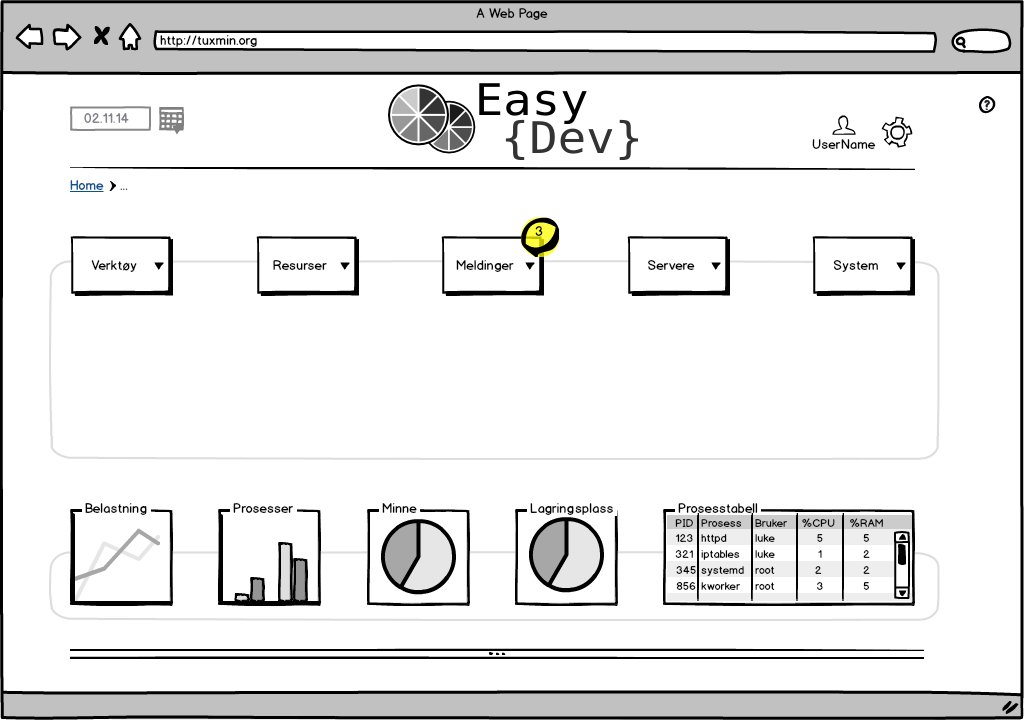
\includegraphics[width=\textwidth,height=\textheight,keepaspectratio]{./img/prosessdokumentasjon/lowfi/fremside.png}
\caption[Low-fi prototype]{Fremside for EasyDev i første low-fi prototype.}
\label{fig:lowfi_fremside}
\end{figure}


I de neste avsnittene beskrives det i detalj funksjonaliteten til de to nevnte modulene. De er begge grunnleggende moduler for systemet som har vært viktige grunnstener som prosjektet ble bygget ut fra. Disse modulene er gode eksempler på hvordan det er tenkt at produktet skal fungere.

\subsection{Oppsett av apache webserver}
Her gås det nærmere inn på hvordan det er tenkt at modulen for konfigurasjon og oppsett av apache webserver gjøres. Alle trinn som beskrives er presentert i figur \ref{fig:lowfiapache}.
Det tas utgangspunkt i at det er intuitiv å velge modul \texttt{Servere} dersom man ønsker å konfigurere en tjener. Modulen er tilgjengelig på fremsiden med en nedtrekksmeny som viser hvilke servere som en har mulighet til å konfigurere, figur \ref{fig:apache1}. 
\textit{Apache} webserver trenger å vite hvilke mapper det skal leses fra. Hvis man installerer apache på en Linux manskin vil den som standard lese fra mappe \texttt{/var/www/} som kun har \texttt{root}-tilgang. Disse rettighetene bør ikke endres ettersom det vil stride mot standarden for rettigheter i systemet og utgjøre en sikkerhetsrisiko.\cite{book:unixprog}
I stedet ønskes det at man definerer om innstillingene i \textit{Apache} slik at serveren leser fra brukerens sin egen mappe. Dette er normalt en utfordring ettersom det må gjøres i form av to til tre trinn\footnote{Antall trinn her er ganske avhengig av hvilken Linux distribusjon som brukes}:

\begin{enumerate}
\item Endre konfigurasjon i apache.conf til å i stedet lese fra brukerens hjemmemappe. Det må opprettes en spesifikk mappe f.eks. \texttt{/home/bruker/html/}. 
I noen tilfeller er det nødvendig å installere plugin \href{http://httpd.apache.org/docs/2.2/mod/mod_userdir.html}{\texttt{mod\_{}userdir}}. Dette vil gjøre det mulig å lese filene med følgende adresse: \texttt{http://localhost/\~{}bruker/fil.html}

\item Endre rettigheter til den mappe i hjemmemappe som filene skal leses fra. Dette forutsetter at brukeren og \textit{Apache} webserver er i samme brukergruppe. Oftest må brukeren bli lagt til \texttt{www}- eller \texttt{httpd}-gruppen i systemet. Det er selvfølgelig mulig å gi rettigheter for mappen til alle grupper i systemet men en slik tilnærming reduserer sikkerheten i stor grad i et flerbrukersystem. Dette er noe som lager en del vanskeligheter for nybegynnere, der man i starten faktisk velger gi alle brukere og gruppe fulle  rettigheter til mappen. 

\item Systemer som benytter seg av SELinux (\href{http://en.wikipedia.org/wiki/Security-Enhanced_Linux}{\textit{Security Enhanced Linux}}) må i tillegg legge til en policy der \textit{Apache} skal få lov til å lese fra brukermapper. Dette er på grunn at SELinux er et oppsett av rettigheter som overstyrer vanlige skrive- og leserettigheter i systemet på kjernenivå\footnote{Dette er ikke noe som beskrives i detalj og blir nevnt her kun for å illustrere problemstillingen som brukeren kan bli utsatt for}. 
\end{enumerate}

Eksemplene ovenfor viser hvor vanskelig det kan være å sette opp Apache webserver på sin egen maskin. Man kunne laget en liknende liste med utfordringer for alle skjermbildene som som presenteres i prosjektet. Med andre ord hvert enkelt bilde i representerer et ukjent antall oppgaver som kjøres i bakgrunnen på systemet, noe som en bruker må utføre helt manuelt dersom de ikke benytter seg av EasyDev.
Dette er et godt eksempel på hvor EasyDev kommer inn med gode løsninger. 

\textit{Apache}-modulen i EasyDev vil alle disse oppgavene for å få en fungerende server.
Dersom man ser i figur \ref{fig:apache2} ser man at under oppsettet kan brukeren velge hvilke mapper som skal inkluderes i konfigurasjonen. Dette er mapper som webserveren vil kunne lese fra. 
I neste trinn (figur \ref{fig:apache3}) blir brukeren bli presentert for hvilken av de valgte mappene man ønsker å aktivere <<\textit{directory browsing}>> på. Det er en funksjon som gjør det mulig å se innholdet i mappen direkte i nettleseren. Dette er normalt en funksjon som ikke brukes på en <<live>> server men er meget bra ved både utvikling og testing.
 
Figur \ref{fig:apache4} viser hvilke typer av plugins som kan legges til \textit{Apache}-installasjonen. Disse kan for eksempel være plugins som PHP eller MySQL eller andre. Hensikten er at man kan samle alle slike tillegg på én plass slik at brukeren kan velge disse ved et senere tidspunkt.
Siste eksempel (figur \ref{fig:apache5}) viser mulighet for konfigurasjon av noen av de mer avanserte tilleggsmoduleene. Det kan f.eks. være støtte for flere virtuelle servere av Apache noe som gir bedre skalerbarhet ved utvikling av flere prosjekter parallelt. 
% med flagg p setter vi hele denne figuren på en egen side
\begin{figure}[p]
        \centering
        \begin{subfigure}[b]{0.48\textwidth}
                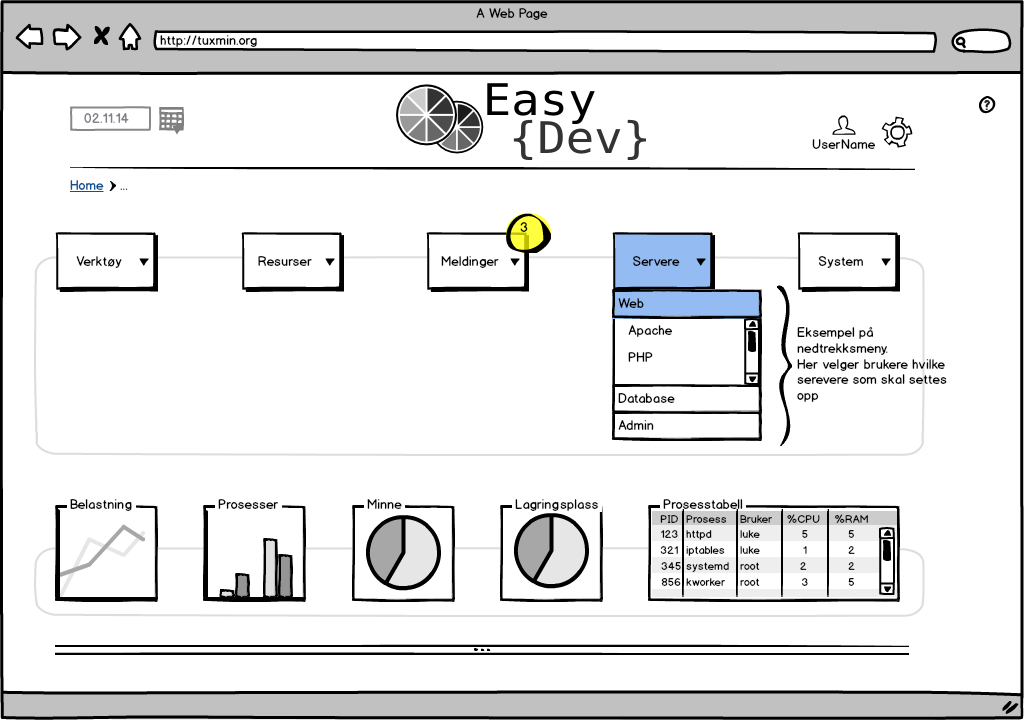
\includegraphics[width=\textwidth]
                {./img/prosessdokumentasjon/lowfi/apache1.png}
                \caption{Fremside -> Sett opp webserver}
                \label{fig:apache1}
        \end{subfigure}
        \begin{subfigure}[b]{0.48\textwidth}
                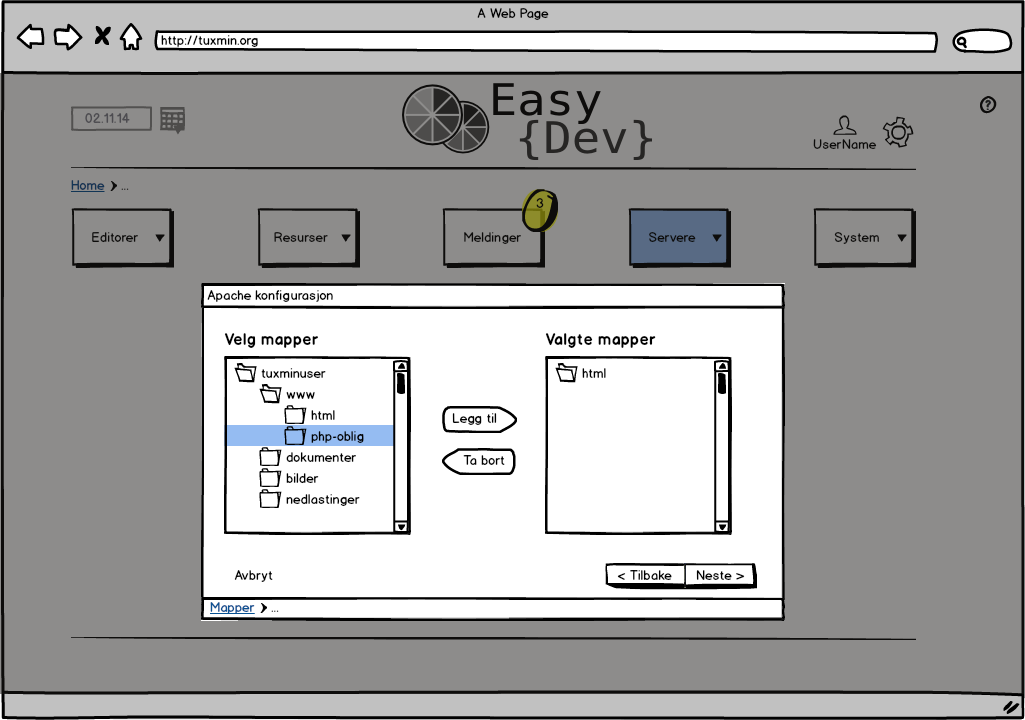
\includegraphics[width=\textwidth]
                {./img/prosessdokumentasjon/lowfi/apache2.png}
                \caption{Valg av mapper}
                \label{fig:apache2}
        \end{subfigure}
       
        \vspace{0.6cm}
        \begin{subfigure}[b]{0.48\textwidth}
                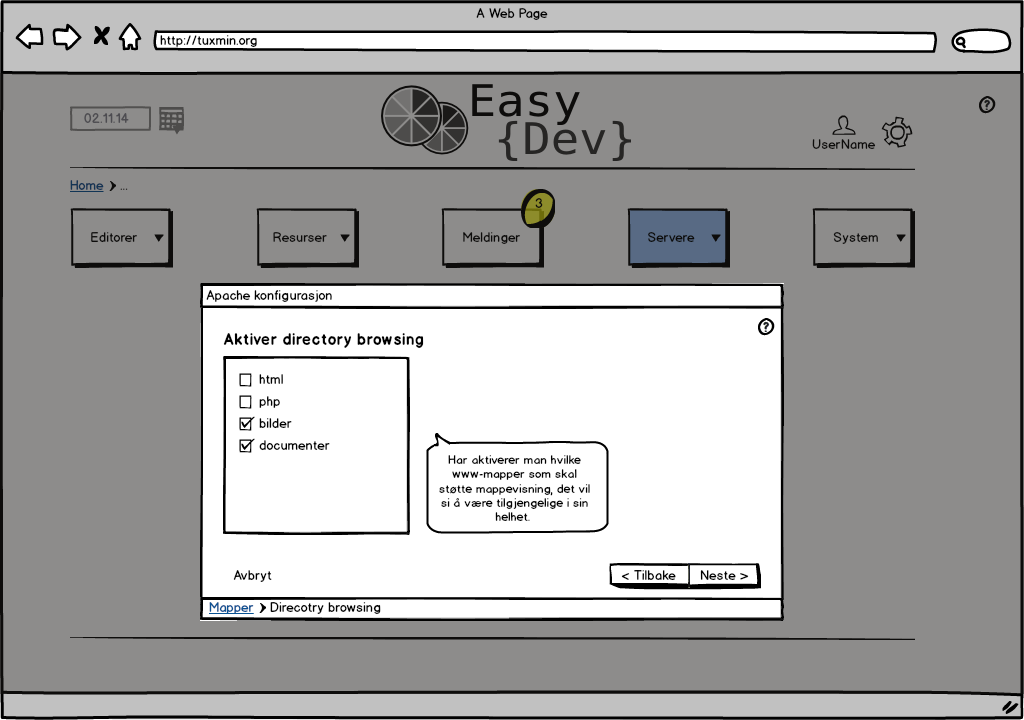
\includegraphics[width=\textwidth]
                {./img/prosessdokumentasjon/lowfi/apache3.png}
                \caption{Aktivere visning av innhold i mapper}
                \label{fig:apache3}
        \end{subfigure}
        %\hspace{0.05cm}
        \begin{subfigure}[b]{0.48\textwidth}
                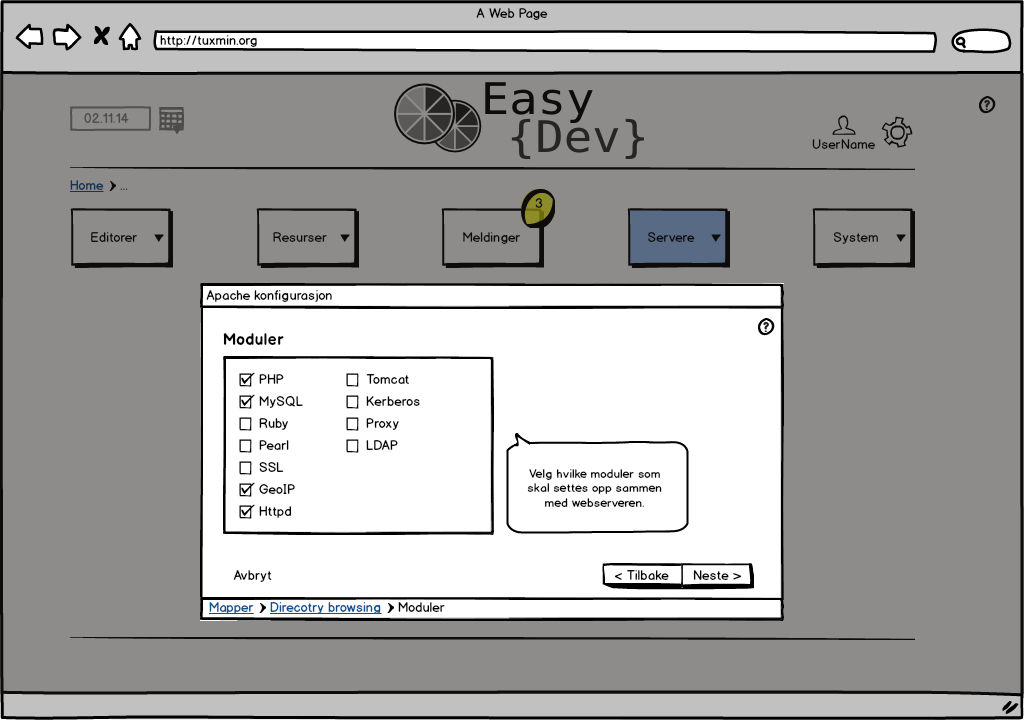
\includegraphics[width=\textwidth]
                {./img/prosessdokumentasjon/lowfi/apache4.png}
                \caption{Valg av moduler}
                \label{fig:apache4}
        \end{subfigure}
        
        \vspace{0.6cm}
        \begin{subfigure}[b]{0.48\textwidth}
                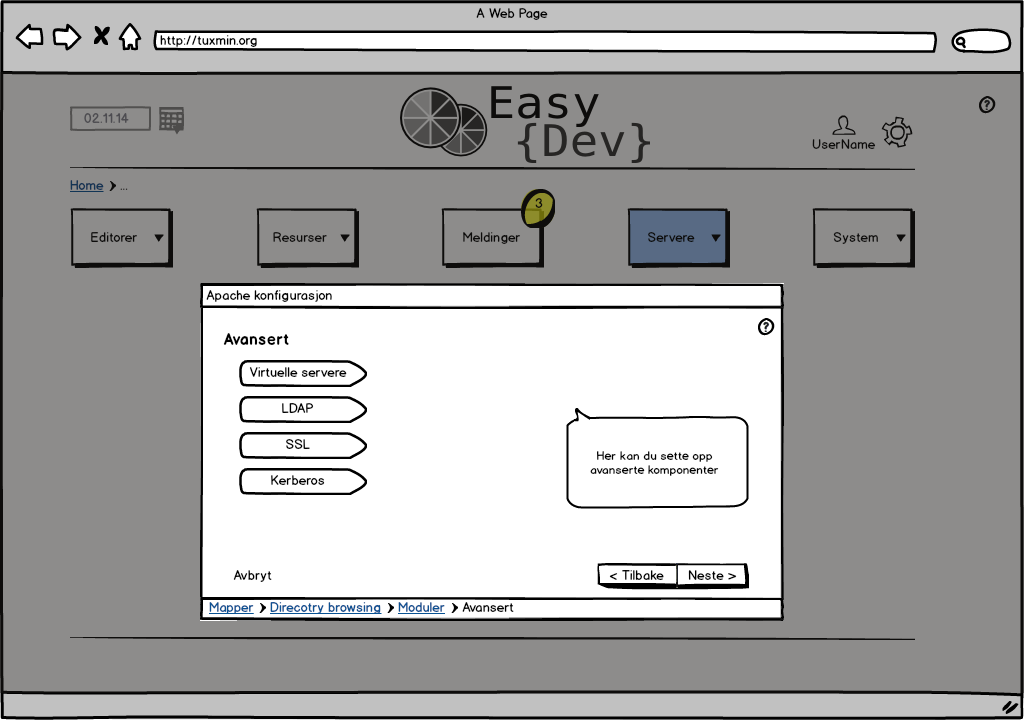
\includegraphics[width=\textwidth]
                {./img/prosessdokumentasjon/lowfi/apache5.png}
                \caption{Avanserte Apache moduler}
                \label{fig:apache5}
        \end{subfigure}
        \vspace{0.1cm}
        \caption[Konfigurasjon av Apache webserver]{Eksempler på konfigurasjon av Apache webserver.}\label{fig:lowfiapache}
\end{figure}

\pagebreak
\subsection{Oppsett av brukere og grupper}
I følgende modul har man mulighet til å konfigurere grupper og brukere samt rettigheter for disse. Modulen er tenkt brukt  der man ønsker å  benytte systemet til gruppearbeid slik at flere brukere kan dele på de samme resursene. De eksemplene som beskrives her finner man i figur \ref{fig:lowfibrukere}. 
% med flagg p setter vi hele denne figuren på en egen side
\begin{figure}[h]
        \centering
        %\hspace*{-0.02\textwidth}
        \begin{subfigure}[b]{0.48\textwidth}
                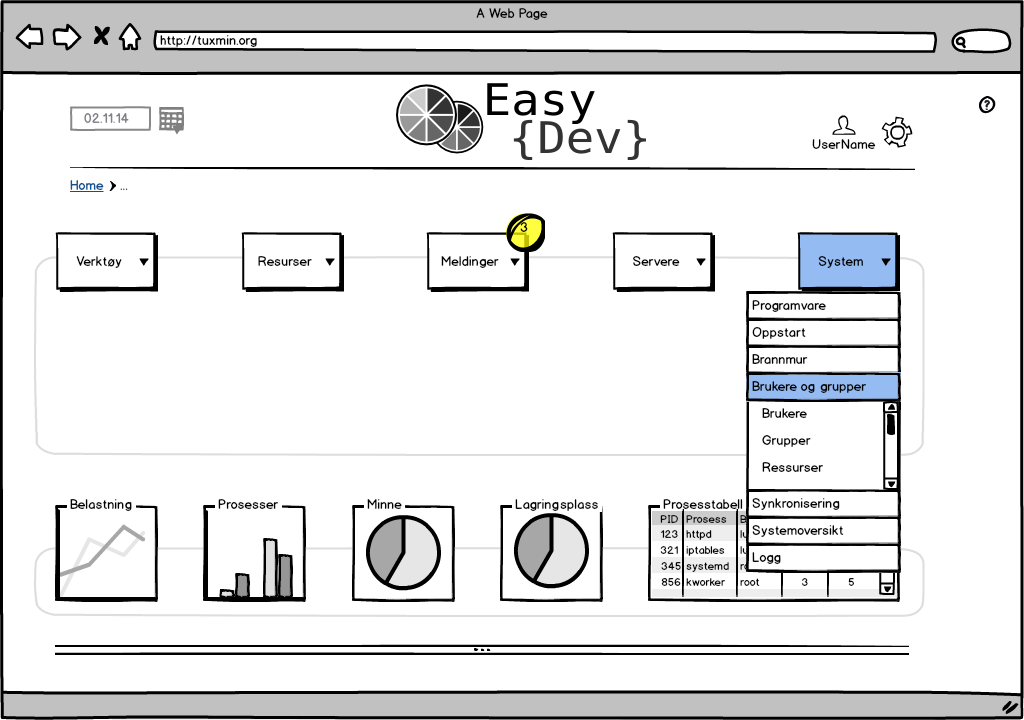
\includegraphics[width=\textwidth]
                {./img/prosessdokumentasjon/lowfi/b1.png}
                \caption{Fremside -> Velg brukeroppsett}
                \label{fig:brukere1}
        \end{subfigure}
        \begin{subfigure}[b]{0.48\textwidth}
                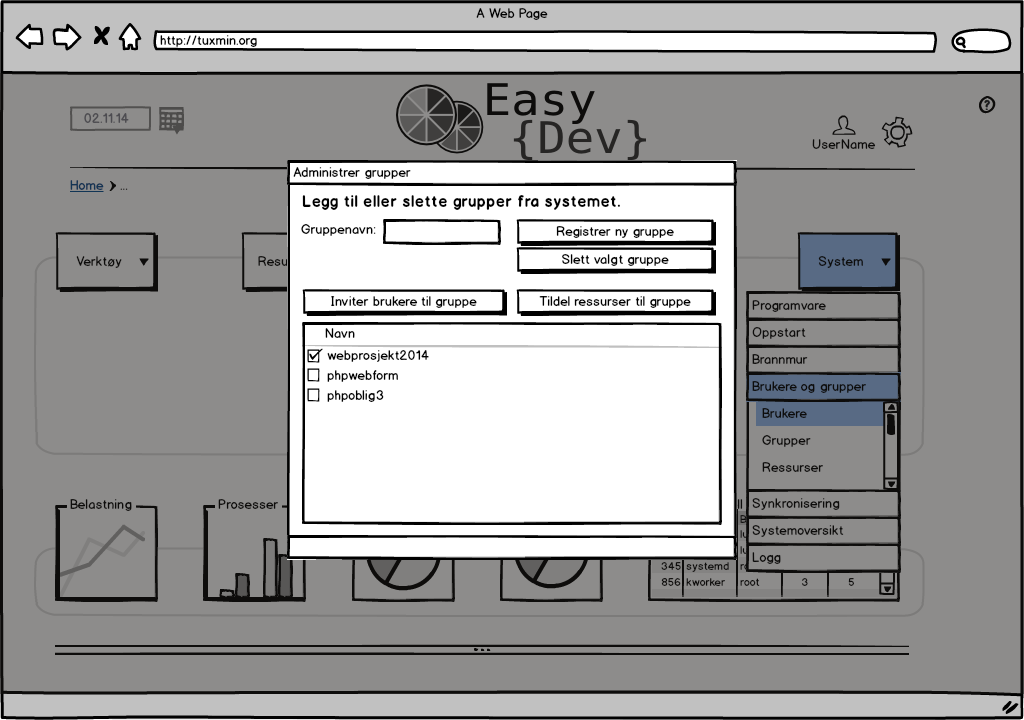
\includegraphics[width=\textwidth]
                {./img/prosessdokumentasjon/lowfi/b2.png}
                \caption{Grupper}
                \label{fig:brukere2}
        \end{subfigure}
        
        \vspace*{0.4cm}
       
        \begin{subfigure}[b]{0.48\textwidth}
                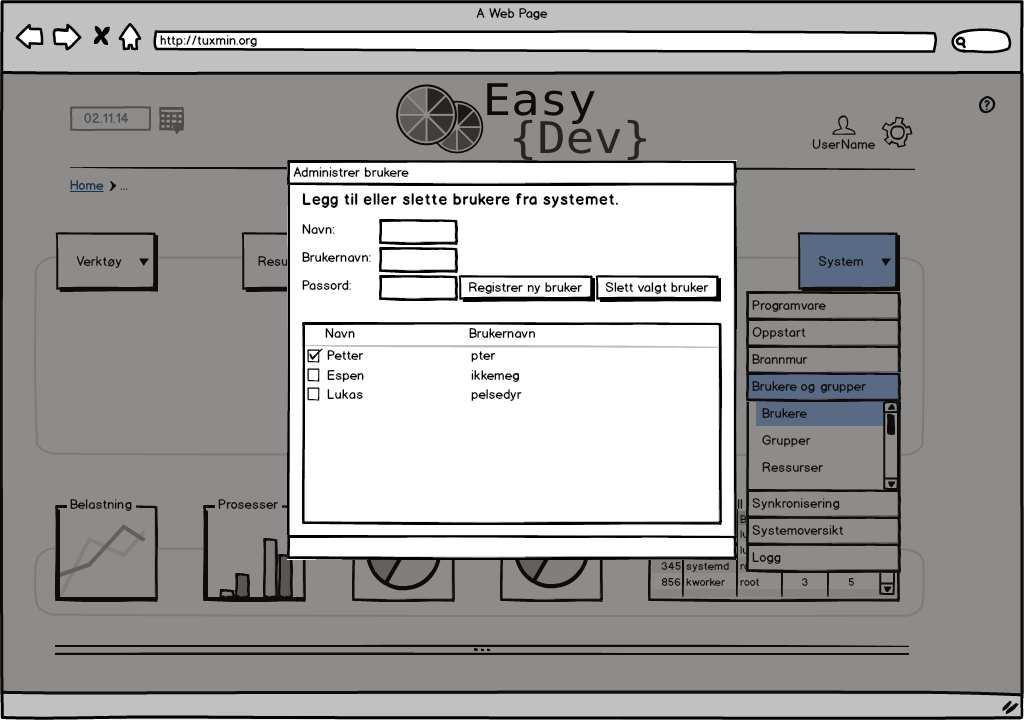
\includegraphics[width=\textwidth]
                {./img/prosessdokumentasjon/lowfi/b3.png}
                \caption{Brukere}
                \label{fig:brukere3}
        \end{subfigure}
        %\hspace{0.02cm}
        \begin{subfigure}[b]{0.48\textwidth}
                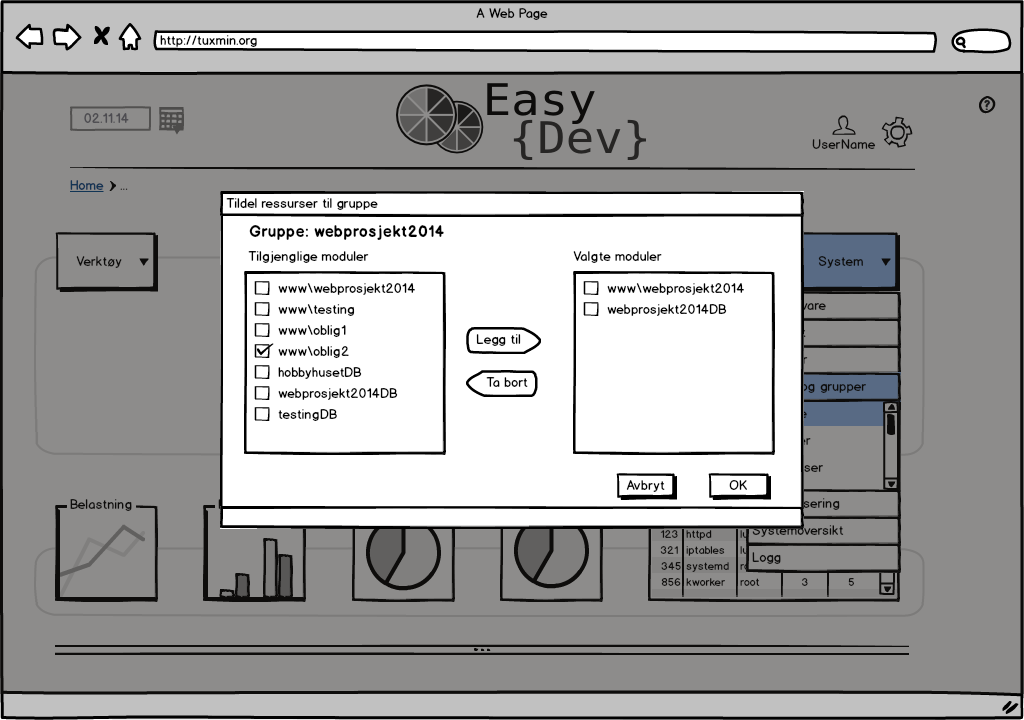
\includegraphics[width=\textwidth]
                {./img/prosessdokumentasjon/lowfi/b4.png}
                \caption{Moduler og ressurser for gruppe}
                \label{fig:brukere4}
        \end{subfigure}
        %\vspace{0.1cm}
        \caption[Konfigurasjon av brukere og grupper]{Eksempel på konfigurasjon av brukere og grupper.}\label{fig:lowfibrukere}
\end{figure}
Som ved forrige eksempel starter  man på fremsiden (figur \ref{fig:brukere1}). I stedet for å velge modul servere går man til modul <<System>> som inneholder flere undermoduler som kan brukes til oppsett og konfigurasjon av selve den virtuelle maskinen og brukergrensesnittet. 
Her (figur \ref{fig:brukere2}) kan det settes opp en ny gruppe, slette gruppe eller gå videre med å legge til brukere til en gruppe. Under knappene ser man også hvilke ressurser som allerede er tildelt den gruppen og eventuelt kan man fjerne disse rettighetene gjennom å fjerne ett eller flere av alternativene.
Dersom man ønsker å legge til nye brukere i systemet kan man gjøre det i neste skjermbilde (figur \ref{fig:brukere3}).
Hvis man ønsker kan man gå videre til neste skjermbilde og legge til nye ressurser som skal være tilgjengelige for en spesifikk gruppe. Dette kan f.eks. dreie seg om en database eller en mappe for webserveren. 

\section{Hi-fi prototype}
\emph{Følgende avsnitt inneholder ikke alle figurer over ferdig hi-fi prototype. Det er mange skjermbilder som må vises i større størrelse for at de skal være lesebare. Samtlige hi-fi mockups er derfor flyttet til appendiks \ref{sec:appendiksHiFi} side \pageref{sec:appendiksHiFi}.}

Hi-fi prototypen er en videreutvikling av tidligere prototype og er laget med hjelp av samme verktøy som skal brukes til utvikling av ferdig produkt. 
Ved utvikling av hi-fi prototype ble det brukt  html, css, javascript og php for å sy sammen funksjonaliteten og få den til å fungere som en nettside. I figur \ref{fig:hifi_fremside} ser man hvordan fremsiden vil kunne se ut. Den kan gjerne sammenliknes med den tidligere mockupen figur \ref{fig:lowfi_fremside} side \pageref{fig:lowfi_fremside} for synliggjøre utviklingsprosessen fra mockup til prototype.
\begin{figure}[ht]
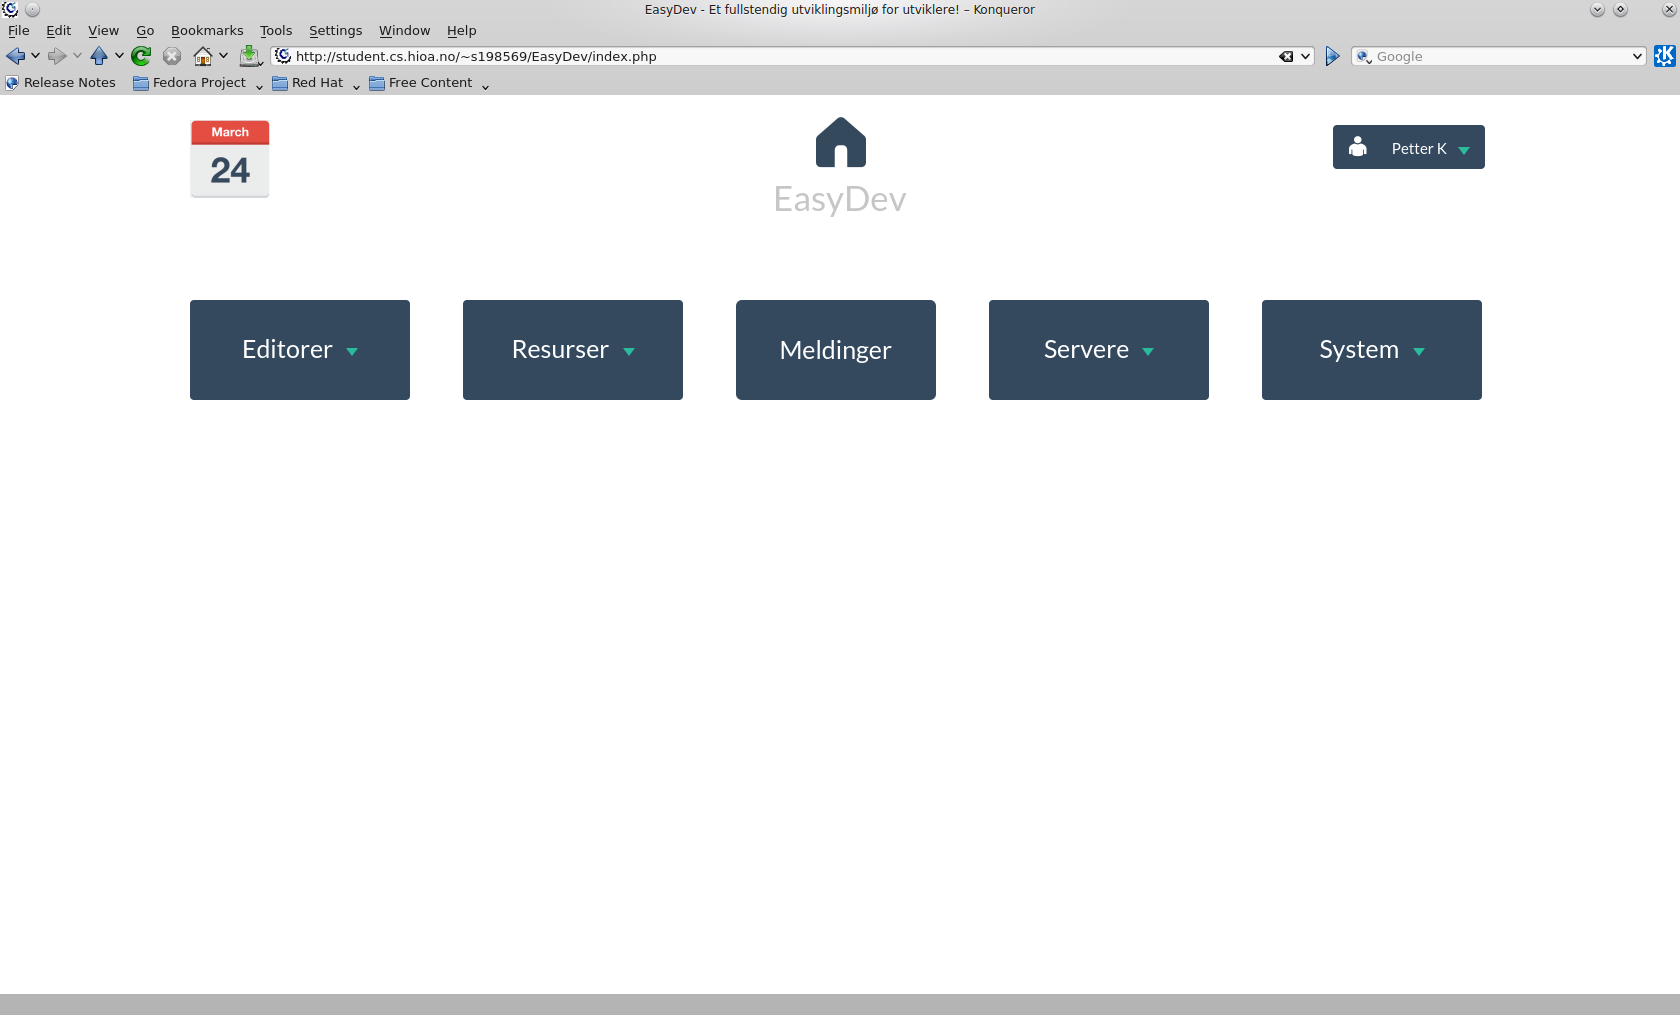
\includegraphics[width=\textwidth,height=\textheight,keepaspectratio]{./img/prosessdokumentasjon/hifi/fremside.png}
\caption[Hi-fi prototype]{Fremside for EasyDev som hi-fi prototype.}
\label{fig:hifi_fremside}
\end{figure}

Det er litt annerledes tilnærming til hvordan dialogvinduene til brukeren blir presentert i hi-fi prototypen. Nærmere eksempel på dette presenteres i figur \ref{fig:hifi_brukerdialog}. 
Vinduene blir presentert lenger ned i forhold til den hovedmenyen. Dette gjør at store deler av det tomme området på fremsiden blir brukt for visning av dialogvinduer. 
Forandringen vil gjøre det mulig for å velge en annen modul direkte uten å behøve avslutte den aktive modulen manuelt (forutsatt at alle endringer som i den aktive modulen er blitt lagret). Den aktive modulen blir da lukket og den nye åpnes.

\begin{figure}[ht]
\centering
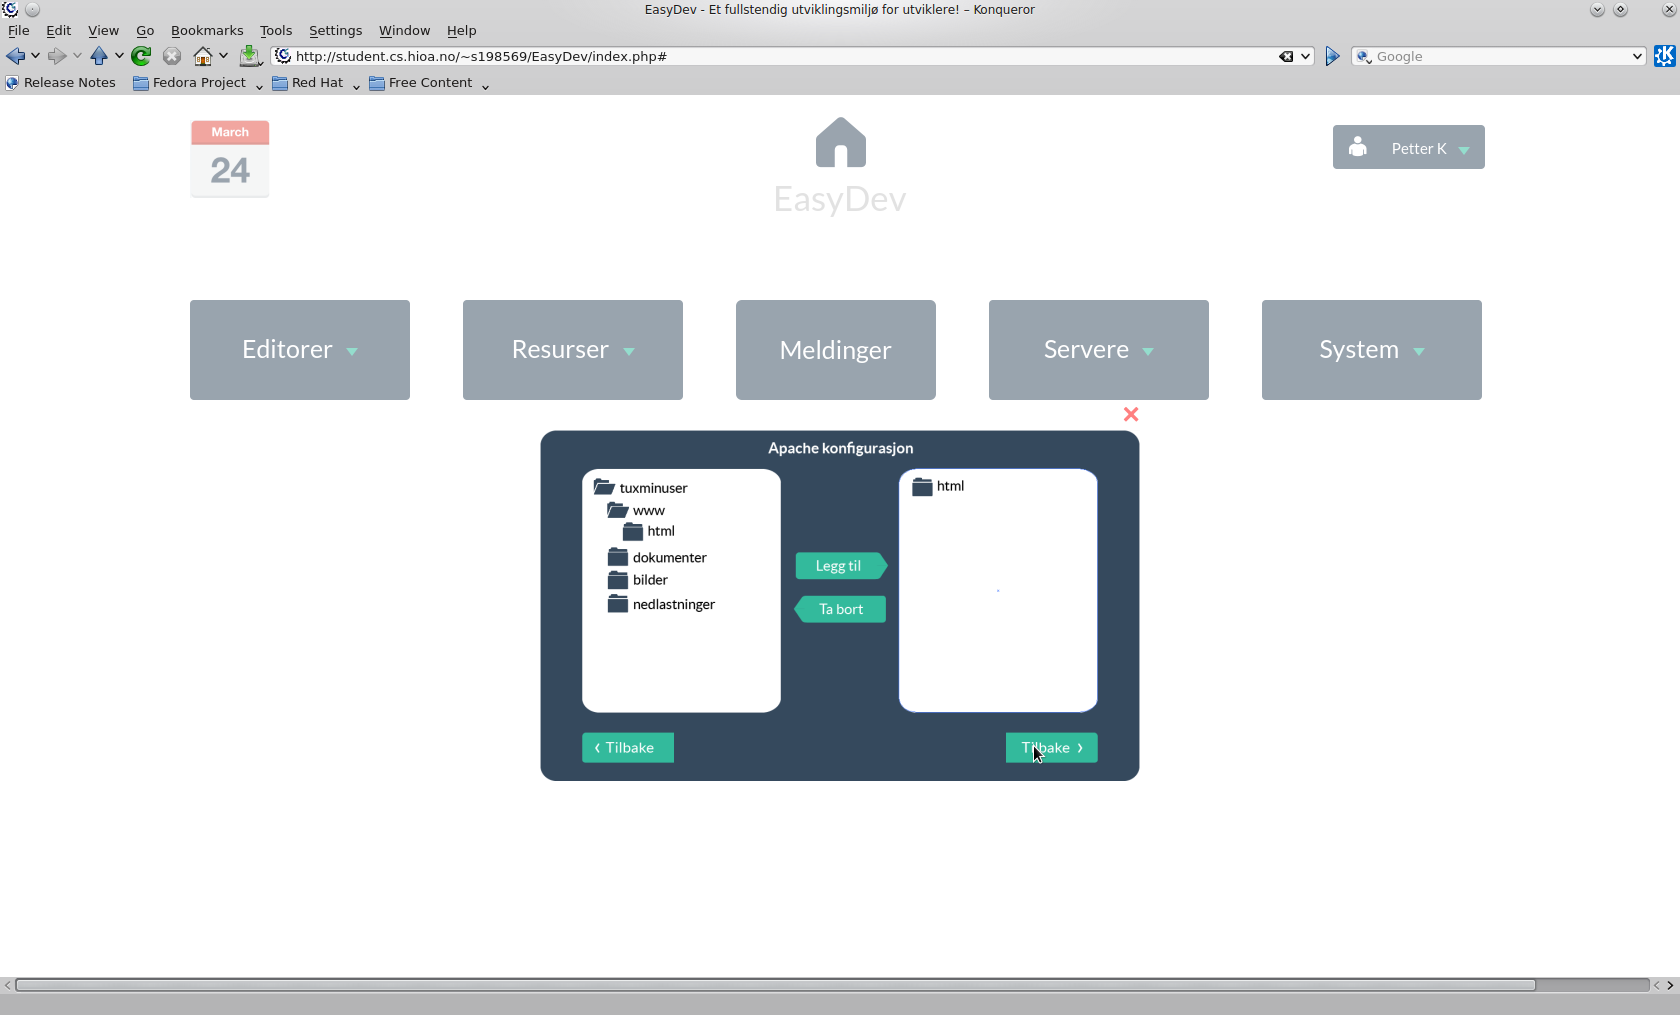
\includegraphics[width=0.8\textwidth,keepaspectratio,trim = {12cm 6cm 12cm 8cm}, clip]{./img/prosessdokumentasjon/hifi/a2.png}
\caption[Hi-fi brukerdialog]{Eksempel på bruker dialogvindu. Utklippet viser eksempel på nytt design og hvor dialogen er plassert i forhold til menyen.}
\label{fig:hifi_brukerdialog}
\end{figure}

\section{Kriterier og avgjørelser}
Følgende avsnitt beskriver hvilke kriterier og valg som ble tatt under veis. Det fokuseres på kriterier og valg fra et MMI-perspektiv men det er også viktig å opplyse om andre kriterier av mer teknisk karakter.

\subsection{Virtuell maskin}
System skal kjøre i en virtuell maskin ettersom det er enkelt å både opprette, slette og gjenopprette systemet. Da en ny bruker skal starte en maskin trenger den kun å bli kopiert fra et \textit{image} og satt opp med riktig brukernavn og passord. Dersom brukeren ødelegger noe i maskinen er  det mulig å eksportere konfigurasjonsfiler for valgte moduler og opprette en ny maskin med sammen med eksisterende konfigurasjonfiler, til f.eks. \textit{Apache}.

\subsection{Webbasert}
Ettersom grensesnittet er webbasert er det tilgjengelig fra hvilken datamaskin, fra hvilke helst uavhengig operativsystem eller nettleser. Systemet vil få en god skalerbarhet da det blir enkelt å sette inn eller fjerne moduler. Det vil også være relativ lav terskel for studenter å utvikle egne moduler dersom man synes at noen vesentlige moduler mangler i systemet. 

\subsection{Bruk av visuelle elementer}
Som tidligere beskrevet i avsnitt \ref{sec:utkast} og \ref{sec:lowfi} har ble det valgt at løsningen skal benytte seg av gestalt prinsipper for plassering av alle visuelle komponenter. 
Hensikten med dette er at når brukeren for første gang besøker fremsiden til systemet, skal det være intuitivt å finne frem, uten å behøve tenkte på hvor de forskjellige knapper og menyer er plassert. 

Et godt eksempel på dette er plassering av alle knapper på fremsiden (se figur \ref{fig:hifi_fremside} side \pageref{fig:hifi_fremside}). 
Disse er plassert horisontalt med samme avstand fra hverandre. 
Slik plassering danner tilhørighet, slik at man vet hvilke komponenter som henger sammen (\textit{proximity, element connectedness, similarity}). I tillegg forsterkes dette gjennom at det brukes samme farger på alle de komponentene.\cite{forelesning:tulpesh}
Samme prinsipper gjelder også for undermenyene. Man blir presentert med en liste av muligheter, gruppert etter tilhørighet til sin funksjon. 

Toppanelet er symmetrisk distribuert for å danne en følelse av balanse og sentral perspektiv i layouten. EasyDev logo er plassert i midten og på hver sin side er kalender og klokke til venstre samt brukerikonet og hurtigvalg av innstillinger til høyre.

I bunnen av skjermbildet var tenkt brukt til elementer som har med status av systemet å gjøre, noe som foreløpig ble forkastet i hi-fi prototype. 
Det var tenkt at man direkte etter pålogging kan får en oversikt over cpu og ram bruk, samt tilgjengelig lagringsplass og kjørende prosesser (se mockup figur \ref{fig:lowfi_fremside} side \pageref{fig:lowfi_fremside}). 
Dette er noe som kan være aktuelt for noen av brukerne men det er foreløpig usikkert om slike funksjoner vil være aktivert for standardbrukere og det er derfor ikke implementert i hi-fi prototype. Det finnes også forslag at plassen kan reserveres til andre formål som brukeren kan selv velge definer, som <<widgets>>. Dette er tilleggsfunksjonalitet som i stor grad bli forandret fra utvikling av prototype til alfa versjon.

\subsection{Bruk av farger}
Det er konsekvent valgt å avgrense farger til grunnpaletten i \textit{FlatUI} grensesnittet. Alle farger som brukes i løsningen ser man i form av en matrise i figur \ref{fig:farger}. Dette er $4\times 5$ matrise som kun har tilgang til tjue farger men gir ganske mange muligheter. 
\begin{figure}[h]
\begin{tabularx}{\textwidth}{*6{>{\centering\arraybackslash}X}@{}}

\cellcolor{Turquoise} \emph{Turquoise} & \cellcolor{Emerald} \textit{Emerald} & \cellcolor{PeterRiver} \emph{Peter River} & \cellcolor{Amethyst} \emph{Amethyst} & \cellcolor{WetAsphalt} \emph{Wet Asphalt} \\[5ex] 

\cellcolor{GreenSea} \emph{Green Sea} & \cellcolor{Nephritis} \textit{Nephritis} & \cellcolor{BelizeHole} \emph{Belize Hole} & \cellcolor{Wisteria} \emph{Wisteria} & \cellcolor{MidnightBlue} \emph{Midnight Blue} \\[5ex] 

\cellcolor{SunFlower} \emph{Sun Flower} & \cellcolor{Carrot} \textit{Carrot} & \cellcolor{Alizarin} \emph{Alizarin} & \cellcolor{Clouds} \emph{Clouds} & \cellcolor{Concrete} \emph{Concrete} \\[5ex] 
 
\cellcolor{Orange} \emph{Orange} & \cellcolor{Pumpkin} \textit{Pumpkin} & \cellcolor{Pomegranate} \emph{Pomegranate} & \cellcolor{Silver} \emph{Silver} & \cellcolor{Asbestos} \emph{Asbestos} \\[5ex] 

\end{tabularx} 
\caption[Fargekombinasjoner]{Fargekombinasjoner som brukes i hi-fi prototypen}
\label{fig:farger}
\end{figure}
Dersom man ser på de to øverste og to nederste radene ser an at disse er forskjellige nyanser av samme farge. Disse er valgt som utheving eller for å danne lav kontrast mellom feks. tabellrader. 

Dersom man trenger mer kontrast for å varsle brukeren om noe kan man ta i bruk to \textbf{analoge} farger. Disse er plassert over hverandre i radene 1-3 eller 2-4, f.eks. \emph{Turqoise} og \emph{Sun Flower} eller \emph{Belize Hole} og \emph{Pomegranade}.
Disse gir myke overganger og kan benyttes sammen for gi en myk overgang f.eks. mellom bakgrunnen i et grensesnitt og et element som kan eksempelvis være en knapp.

Til sist er det også mulig å benytte seg av to \textbf{komplementærfarger}.
Disse har er plassert på skrå fra hverandre som \emph{Peter River} og \emph{Orange} eller \emph{Amethyst} og \emph{Sun Flower}. Disse fargene, hvis de brukes sammen, gi en tydelig markering mellom de komponentene som fargene representerer. 
Alle disse fargene er selvsagt ikke benyttet i hi-fi prototypen da mange av dem blir reservert til spesielle tilfeller. Kun mer monotone av farger i figur \ref{fig:farger} blir brukt til komponenter og bakgrunner som ofte forekommer i komponentene.

\subsection{Open Source}
Løsningen er kun basert på produkter som er tilgjengelige via open source eller som fri kode. Dette er ganske kritisk da prosjektet, om det videreutvikles, ikke skal være avhengig av proprietær teknologi.
Prosjektet komme til å være åpnet tilgjengelig slik at det kan opprettes såkalte <<forks>> av dem som ønsker videreutvikle det i en annen retning.